\begin{figure}[htbp]
\centering
\begin{tikzpicture}[x=1cm,y=1cm]
\node[anchor=south west,inner sep=0] at (0,0) {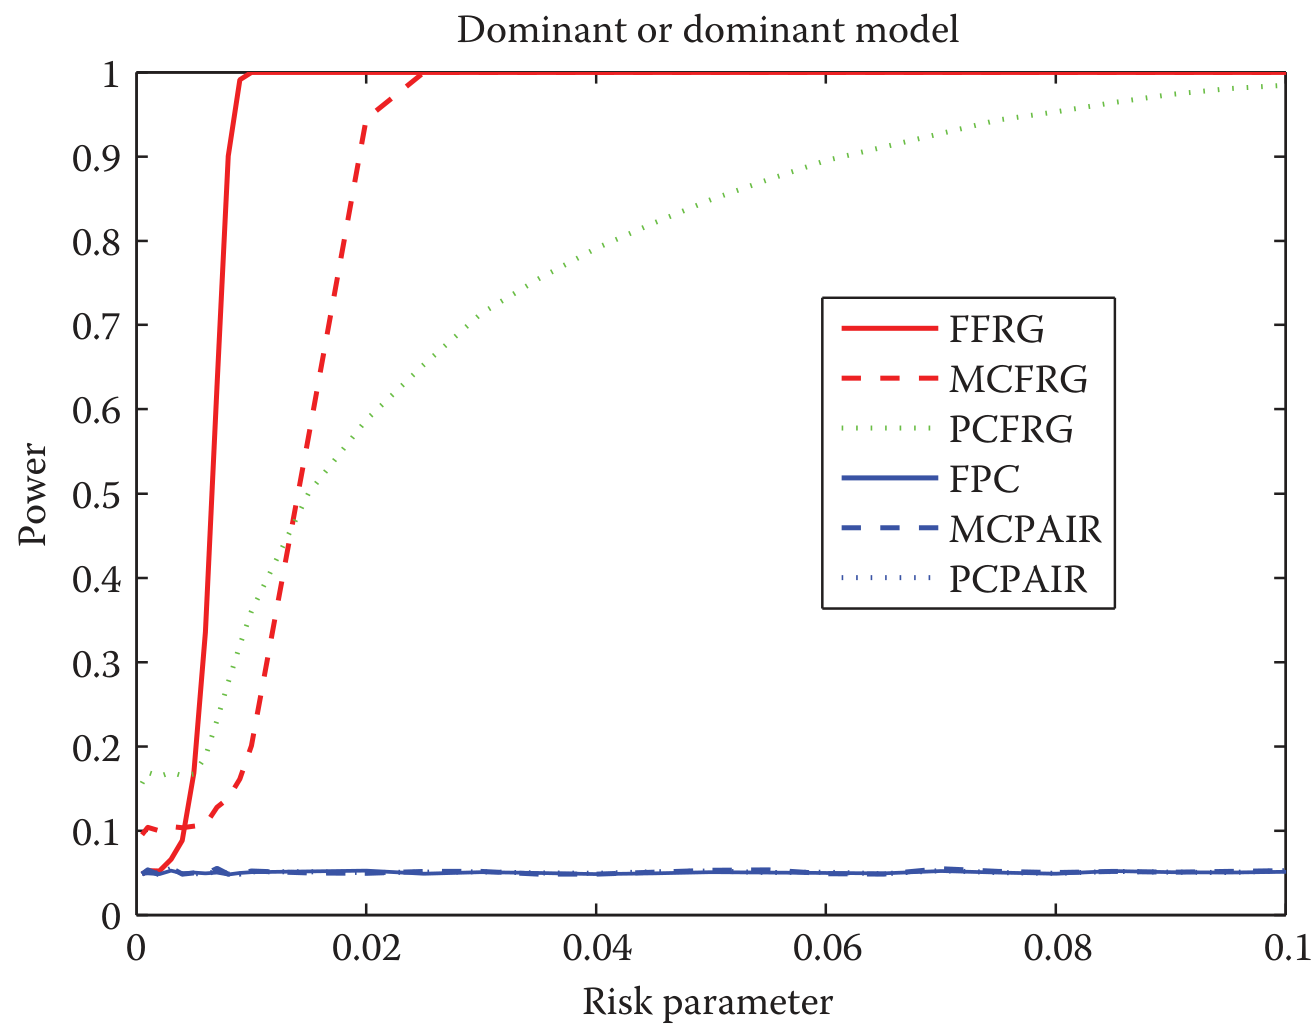
\includegraphics[width=13.8cm]{figures/ch03_fig23_data.png}};
\fill[white] (6.0740,0.0415) rectangle (8.7836,0.5138);
\node[font=\small,rotate=0,inner sep=0] at (7.4288,0.2776) {风险参数};
\fill[white] (0.1256,5.0373) rectangle (0.6084,6.1972);
\node[font=\small,rotate=90,inner sep=0] at (0.3670,5.6172) {统计功效};
\fill[white] (4.7583,10.2349) rectangle (10.0994,10.7071);
\node[font=\small,rotate=0,inner sep=0] at (7.4289,10.4710) {显性或显性模型};
\end{tikzpicture}
\origfig{23}{显性或显性模型下六种统计量 F-FRG、MC-FRG、PC-FRG、FPC-FPC、PC-pair-wise 和 MC-pair-wise 的功效曲线。}
\label{fig:ch03-23}
\end{figure}
